\chapter{Revisão bibliográfica}

\section{Estacionariedade}
		
Nesta seção são apresentadas as definições de funções aleatórias e estacionariedade. Fundamentais ao pleno entendimento da necessidade da modelagem dos domínios geológicos de um depósito mineral sob o ponto de vista matemático. \cite{matheron1965variables, journel1978mining, armstrong1998basic}.
	
\subsection{Funções aleatórias}\label{func_al}
			
Um fenômeno natural pode muitas vezes ser caracterizado pela distribuição espacial de uma ou mais variáveis, chamadas variáveis regionalizadas (ReV).
			
Uma variável aleatória (RV), é uma variável que recebe um certo número de valores numéricos de acordo com uma determinada distribuição de probabilidade. O resultado do lançamento de um dado, por exemplo, pode ser considerado uma RV que pode receber um entre seis valores equiprováveis. 
			
Um valor observado em um ponto amostral $x_i$ é  a realização, $z(x_i)$ de uma variável regionalizada, $Z(x_i)$. A família de todas as variáveis aleatórias auto-correlacionadas $Z(x)$ quando $x$ varia por todo o domínio ($D$) de um depósito é uma função aleatória (RF) $\{Z(x),x\in D\}$. Essa definição de função aleatória expressa o aspecto aleatório e estruturado das variáveis regionalizadas.

Localmente, no ponto $x_i$, $Z(x_i)$ é uma variável aleatória. $Z(x)$ é uma RF, já que para cada par de pontos $x_i$ e $x_i+h$, as RV correspondentes, $Z(x_i)$ e $Z(x_i+h)$ não são independentes, são relacionadas por uma correlação que expressa a estrutura espacial da variável regionalizada $z(x)$.
			 
De acordo com \citeonline{journel1978mining}, o problema então, passa a ser representar a variabilidade da função aleatória no espaço (quando $x$ varia), essa representação será usada para resolver problemas de estimativa do valor $z(x_0)$ em um ponto $x_0$ que não foi amostrado.
			
A interpretação probabilística da Variável regionalizada $z(x)$ como sendo uma determinada realização de uma certa RF $Z(x)$ faz sentido apenas quando é possível inferir, mesmo que parcialmente, a lei de probabilidade que define a RF.
			
É virtualmente impossível inferir a lei de probabilidade de uma RF $Z(x)$ a partir de uma única realização $z(x)$, que por sua vez é limitada a um número finito de pontos amostrais $x_i$. Da mesma forma, é impossível determinar a lei de probabilidade que rege o lançamento de um dado a partir do resultado de um único lançamento, vários lançamentos são necessários para sua determinação. Várias realizações $z_1(x),z_2(x),...,z_k(x)$ da RF $Z(x)$ seriam necessárias para inferir a lei de probabilidade de $Z(x)$, na prática estamos limitados a uma única realização $\{z(x_i)\}$ da RF nas posições $x_i$, então, certas suposições envolvendo graus de homogeneidade espacial devem ser estabelecidas, a hipótese de estacionariedade.
			
Na prática, mesmo que apenas certa região do fenômeno possa ser considerada homogênea, a ReV se repete no espaço. Essa homogeneidade ou repetição é equivalente a várias realizações da mesma RF $Z(x)$ e permite certo grau de inferência estatística. Dois pontos experimentais $z(x_0)$ e $z(x_0+h)$ em dois pontos diferentes, $x_0$ e $x_0+h$, podem então, ser tratados como duas realizações da mesma RV $Z(x_0)$. Essa abordagem é usada para inferir a lei de distribuição da RF $Z(x)$ a partir do histograma dos dados $\{z(x_i)\}$, assim como o valor esperado $E\{Z(x)\}$ a partir da média aritmética dos dados.
			
\subsection{Momentos}
		
Considere a RF $Z(x)$. Para cada conjunto de $k$ pontos no $R^n$ (espaço n-dimensional) $x_1,x_2,...,x_k$, corresponde um componente vetorial k-dimensional de variáveis aleatórias  $\{Z(x_1),Z(x_2),...,Z(x_k)\}$.
			
Essa RV vetorial é caracterizada pela função de distribuição (ccdf), condicionada aos $k$ pontos amostrais $F_{x_1,x_2,...,x_k}(z_1,z_2,...,z_k)=Prob\{Z(x_1)<z_1,...,Z(x_k)<z_k\}$.
			
O conjunto de todas as funções de distribuição, para todos os $k$ inteiros e positivos e para todas as escolhas possíveis de pontos no $R^n$, constitui a lei espacial da RF $Z(x)$.
			
Em aplicações na mineração, não é necessário caracterizar toda a lei espacial, apenas os dois primeiros momentos da lei são necessários para uma solução aproximada dos problemas encontrados. Além disso, a quantidade de dados disponível é insuficiente pra inferir a lei espacial em sua totalidade \cite{journel1978mining}.
			
Seguem as definições dos momentos segundo \citeonline{journel1978mining}
			
\subsubsection{Momento de primeira ordem}
				
Considere a RV $Z(x)$ no ponto $x$. Se a função de distribuição de $Z(x)$ tem uma esperança matemática que depende do ponto $x$, essa é:
				
\begin{equation}
	E\{Z(x)\}=m(x)
\end{equation}
                
\subsubsection{Momentos de segunda ordem}
			
Na geoestatística, os momentos de segunda ordem são:
				

A variância, ou mais precisamente, variância \textit{a priori} de $Z(x)$, é definida como o momento de segunda ordem em relação a esperança $m(x)$ da RV $Z(x)$,

\begin{equation}
	Var\{Z(x)\}=E\{[Z(x)-m(x)]^2\}
\end{equation}	

A covariância. Pode ser demonstrado que se duas RV $Z(x_1)$ e $Z(x_2)$ têm variâncias nos pontos $x_1$ e $x_2$ elas também têm uma covariância, que é função das duas localidades $x_1$ e $x_2$, e pode ser escrita como:
				
\begin{equation}
	C(x_1,x_2)=E\{[Z(x_1)-m(x_1)][Z(x_2)-m(x_2)]\}
\end{equation}

O variograma, que é definido como a variância do incremento $[Z(x_1)-Z(x_2)]$, pode ser escrito como:
				
\begin{equation}
	2\gamma(x_1,x_2)=Var\{Z(x_1)-Z(x_2)\}
\end{equation}
				
A função $\gamma(x_1,x_2)$ é o semi-variograma.
				
\subsection{Hipótese de estacionariedade}
		
Por definição, funções variograma e covariância dependem simultaneamente de dois pontos $x_1$ e $x_2$, então várias realizações do par de RV $\{Z(x_1),Z(x_2)\}$ são necessários para que qualquer inferência estatística seja possível.
			
Por outro lado, se essas funções dependerem somente da distância entre dois pontos, isto é, do vetor $h=x_1-x_2$ que separa $x_1$ e $x_2$, a inferência estatística se torna possível. Cada par de dados $\{z(x_k),z(x_{k'})\}$ separados pela distância $(x_k-x_{k'})$, igual ao vetor $h$, pode ser considerado como uma realização diferente do par de RV $\{Z(x_1),Z(x_2)\}$.
			
É intuitivo perceber que em zonas de mineralização homogêneas (domínios geológicos), a correlação que existe entre dois pontos $z(x_k)$ e $z(x_{k'})$ não depende das posições dentro dessas zonas homogêneas, mas da distância que os separa.
			
\citeonline{journel1978mining} apresentam diferentes tipos de estacionariedade. 
		
\subsubsection{Estacionariedade estrita}
				
Uma RF é dita estacionária estrita quando sua lei espacial é invariante à translação. As duas componentes vetoriais $\{Z(x_1),Z(x_k)\}$ e $\{Z(x_1+h),Z(x_k+h)\}$ têm a mesma lei de distribuição, independente do vetor de translação $h$.
				
Na geoestatística linear, estamos interessados apenas nos dois primeiros momentos, então será necessário assumir a estacionariedade apenas para eles.
				
\subsubsection{Estacionariedade segunda ordem}
			
Uma RF é dita estacionária de segunda ordem quando sua esperança matemática existe e não depende do ponto x.

\begin{equation}
	E\{Z(x)\}=m, \quad \forall x
\end{equation}
					
A média de $Z(x)$ é a média do domínio geológico estacionário.
					
Para cada par de RV $\{Z(x),Z(x+h)\}$, a covariância existe e depende da distância de separação $h$.
					
\begin{equation}
	C(h)=E\{Z(x_h)Z(x)\}-m^2, \quad \forall x
\end{equation}
					
$h$ representa um vetor de coordenadas no espaço tridimensional.
					
Sob a hipótese de estacionariedade de segunda ordem $\gamma(h)=C(0)-C(h)$.
			
\subsubsection{Hipótese intrínseca}
				
Uma RF $Z(x)$ é dita intrínseca quando sua esperança matemática existe e não depende do ponto x.
				
\begin{equation}
	E\{Z(x)\}=m, \quad \forall x
\end{equation}
				
A média de $Z(x)$ é a média do domínio geológico estacionário.

Para todos os vetores $h$ o incremento $[Z(x+h)-Z(x)]$ tem variância finita que não depende $x$
				
\begin{equation}
	Var\{Z(x+h)-Z(x)\}=E\{[Z(x+h)-Z(x)]^2\}=2\gamma(h), \quad \forall x
\end{equation}
				
Então, a estacionariedade de segunda ordem implica na hipótese intrínseca, mas o contrário não é verdadeiro. A hipótese intrínseca pode ser vista como uma limitação da estacionariedade de segunda ordem aos incrementos da RF $Z(x)$
				
\subsubsection{Quasi-estacionariedade}
			
Na prática, a covariância ou variograma são usados apenas para distâncias limitadas $|h| \le b$, como por exemplo, $b$ poderia ser o diâmetro da vizinhança de busca, em outros casos $b$ pode ser uma zona de mineralização homogênea (domínio geológico) e duas variáveis $Z(x_k)$ e $Z(x_k+h)$ não podem ser consideradas provenientes do mesmo domínio se $|h|>b$.
				
Nesses casos, devemos considerar a função $C(x,x+h)$ ou $\gamma(x,x+h)$ não mais do que localmente estacionárias, para distâncias $|h|$ menores que $b$. Essa limitação da hipótese de segunda ordem é a hipótese de quasi-estacionariedade.
							
\subsection{Decisão de estacionariedade}
				
A decisão de estacionariedade é uma suposição, e requisito a aplicação das técnicas geostatísticas de estimativa e simulação. Estacionariedade não é uma propriedade geológica, é uma propriedade matemática.
				
Uma função aleatória estacionária (SRF) é a representação probabilística de uma propriedade petrofísica com esperança matemática e covariância constantes independe da localização. Raramente, é apropriado considerar a totalidade do depósito mineral como um único domínio estacionário, que será modelado a partir de uma SRF. Geralmente, é necessário identificar diferentes domínios no depósito, cada um com seu modelo de SRF, consistentes com as suposições matemáticas de uma SRF \cite{mclennan}.
				
A \autoref{veio_ouro} mostra um veio mineralizado de quartzo-ouro em rocha encaixante máfica, os teores de ouro se comportam de maneira diferente no veio e rocha encaixante, os teores são mais altos e mais variáveis no veio. Assumir estacionariedade, e modelar com uma única SRF toda a região não seria adequado. O modelo numérico será mais consistente com a realidade se duas SRF forem usadas, uma para cada unidade geológica.
				
\begin{figure}[!htb]
	\caption{\label{veio_ouro}Veio de quartzo-ouro em rocha máfica.}
	\begin{center}
		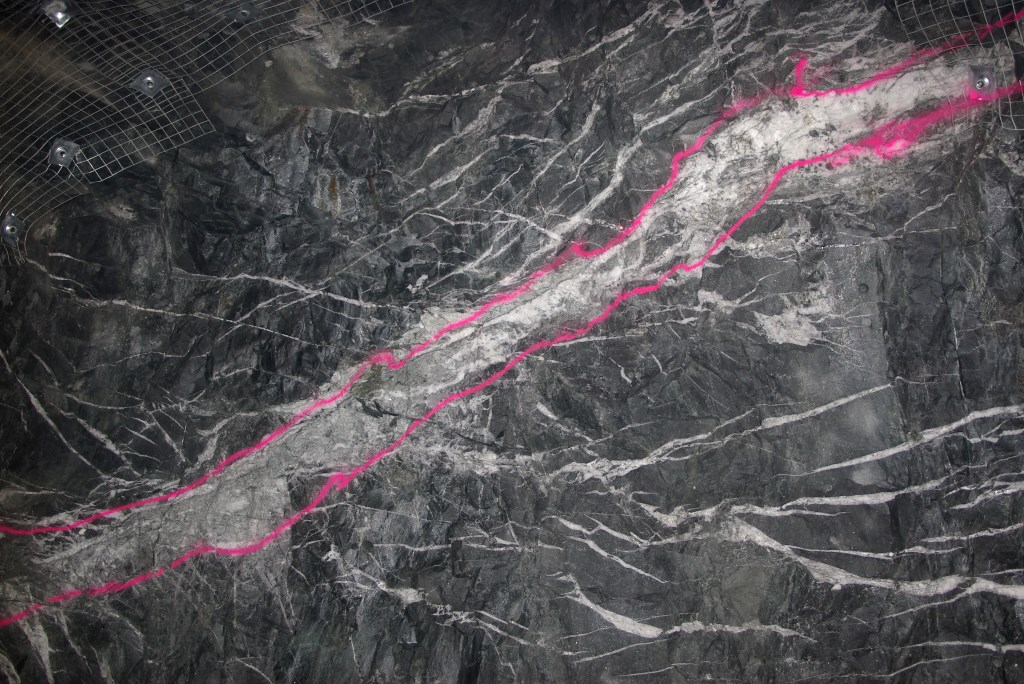
\includegraphics[width=0.6\textwidth]{revisao_bibliografica/veio_ouro.jpg}
	\end{center}
	\legend{Fonte: \url{http://rses.anu.edu.au/people/steve-cox}, acesso em julho de 2016}
\end{figure}
				
Segundo \citeonline{mclennan}, para que a decisão de estacionariedade seja razoável um total de cinco fases devem ser consideradas: 
				
\begin{enumerate}
\item{Escolher o número e tipo dos domínios que terão suas propriedades petrofísicas modeladas;}
\item{Modelar as fronteiras desses domínios;}
\item{Caracterizar a natureza das transições entre os domínios e modelá-las;}
\item{Modelar as tendências (\textit{trends}) dentro de cada domínio;}
\item{Estimar com um modelo de tendência.}
\end{enumerate}
				
A escolha dos domínios deve ser avaliada com base em um equilíbrio entre um modelo geológica e fisicamente consistentes e o número de amostras disponível para inferir os parâmetros das SRF \cite{mclennan}.

Além da imposição matemática, os domínios de um depósito mineral devem ser modelados para que estimativas mais precisas de volume/massa e teores sejam obtidas e problemas de diluição ocasionados pela falta de aderência do modelo de blocos às estruturas geológicas do depósito sejam reduzidos \cite{rasera2014estrati}. 
				
\section{Funções implícitas} \label{sec_func_imp}

Alguns dos métodos determinísticos de modelagem geológica disponíveis, e revisados nessa dissertação, são baseados em funções implícitas. O uso da modelagem implícita foi introduzido no campo da computação gráfica para criação de objetos de diversas geometrias e complexidades por \citeonline{bloomenthal1997introduction}. A ideia central da técnica é usar uma função implícita para demarcar regiões de diferentes formas e extensões no espaço \cite{maureira}.

Na matemática, uma equação implícita é uma relação na forma $R(x_1,...,x_n)=0$. Por exemplo, a equação implícita de um círculo unitário é $x^2+y^2-1=0$.

Uma função implícita é uma função definida implicitamente por uma equação implícita, associando uma das variáveis (o valor) com as outras (os argumentos). A função implícita que define o círculo unitário pode ser escrita como $x^2+f(x)^2-1=0$. Essa equação implícita define $f$ como uma função de $x$ apenas se $-1 \leq x\leq 1$.

Os exemplos a seguir, que ilustram a metodologia, foram propostos por \citeonline{osher}.

Na \autoref{linha}, em uma dimensão, a linha dos números reais foi dividida em três partes distintas usando os pontos $x=-1$ e $x=1$. Isto é, definimos $(-\infty,-1)$, $(-1,1)$ e $(1,\infty)$. A primeira e terceira partes são peças desconexas da mesma região. Assim, definimos $\Omega^-=(-1,1)$ como parte interna do domínio e $\Omega^+=(-\infty,-1)\cup(1,\infty)$ como parte externa do domínio. A fronteira entre a parte interna e externa consiste dos dois pontos $\partial\Omega=\{-1,1\}$, e é chamada de interface. No $\Re^n$, os subdomínios são $n$-dimensionais, enquanto a interface apresenta $n-1$ dimensões.

\begin{figure}[!htb]
	\caption{\label{linha}Linha dos reais dividia em dois subdomínios pelos pontos $x=-1$ e $x=1$.}
	\begin{center}
		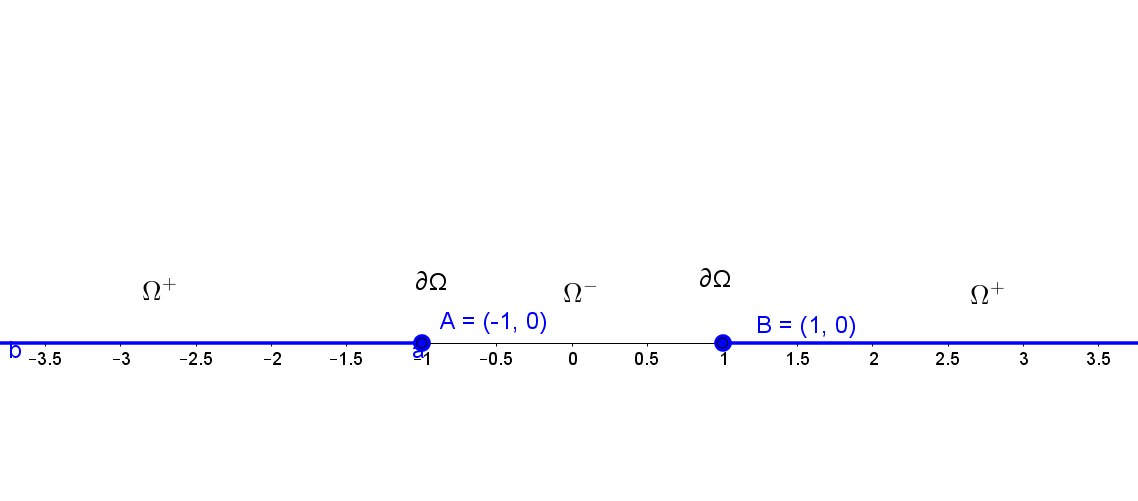
\includegraphics[width=0.6\textwidth]{revisao_bibliografica/linha}
	\end{center}
	%\legend{}
\end{figure}

Numa representação explícita da interface, escrevemos explicitamente os pontos que a definem como feito anteriormente ao definir $\partial\Omega=\{-1,1\}$. Também é possível definir implicitamente a interface como o isocontorno de de alguma função. Por exemplo, o isocontorno zero de $\phi(x)=x^2-1$ é o conjunto de pontos para os quais $\phi(x)=0$, isto é, exatamente $\partial\Omega=\{-1,1\}$, como pode ser observado na \autoref{func}. 

\begin{figure}[!htb]
	\caption{\label{func}Função implícita definindo as regiões $\Omega^-$ e $\Omega^+$ bem como a fronteira $\partial\Omega$.}
	\begin{center}
		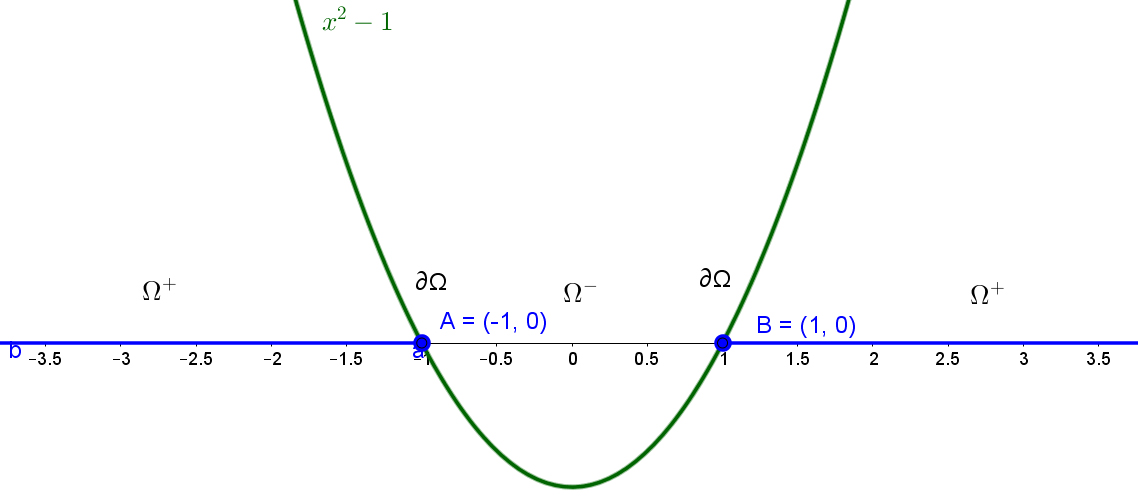
\includegraphics[width=0.6\textwidth]{revisao_bibliografica/funcao}
	\end{center}
	\legend{Modificado de \citeonline{osher}}
\end{figure}

O isocontorno zero foi escolhido. Porém não há nada de especial nessa escolha, o isocontorno $\phi(x)=1$ da função $\phi(x)=x^2$ define a mesma interface.

\subsection{Funções distâncias assinaladas}

Na \autoref{sec_func_imp}, foram definidas as funções implícitas, seu valor é $\phi(x)=0$ na interface, $\phi(x)<0$ na região interna e $\phi(x)>0$ na região externa. As funções distância assinaladas são um subconjunto das funções implícitas.     

Uma função distância $d(\vec{x})$ é definida como:

\begin{equation}
d(\vec{x})=min(|\vec{x}-\vec{x_I}|) \quad \forall \quad \vec{x_I} \in \partial\Omega
\end{equation}

Onde $\vec{x_I}$ é um ponto pertencente à interface. Ou seja, para um dado ponto $\vec{x}$, $d(\vec{x})$ é a menor distância entre $\vec{x}$ e um ponto $\vec{x_C}$ pertencente à interface $\partial\Omega$.   

Uma função distância assinalada é uma função implícita $\phi$, com $|\phi(\vec{x})|=d(\vec{x})$ para todo $\vec{x}$. Então, $\phi(\vec{x})=d(\vec{x})=0$ para todo $\vec{x} \in \partial\Omega$, $\phi(\vec{x})=-d(\vec{x})$ para todo $\vec{x} \in \Omega^-$ e $\phi(\vec{x})=d(\vec{x})$ para todo $\vec{x} \in \Omega^+$.

Na \autoref{sec_func_imp}, a função $\phi(x)=x^2-1$ foi usada para representar implicitamente a interface $\partial\Omega=\{-1,1\}$. Uma representação baseada em funções distância assinaladas da mesma interface é $\phi(x)=|x|-1$, como visto na \autoref{sig_dist} 

\begin{figure}[!htb]
	\caption{\label{sig_dist}Função distância assinalada definindo as regiões $\Omega^-$ e $\Omega^+$ bem como a fronteira $\partial\Omega$.}
	\begin{center}
		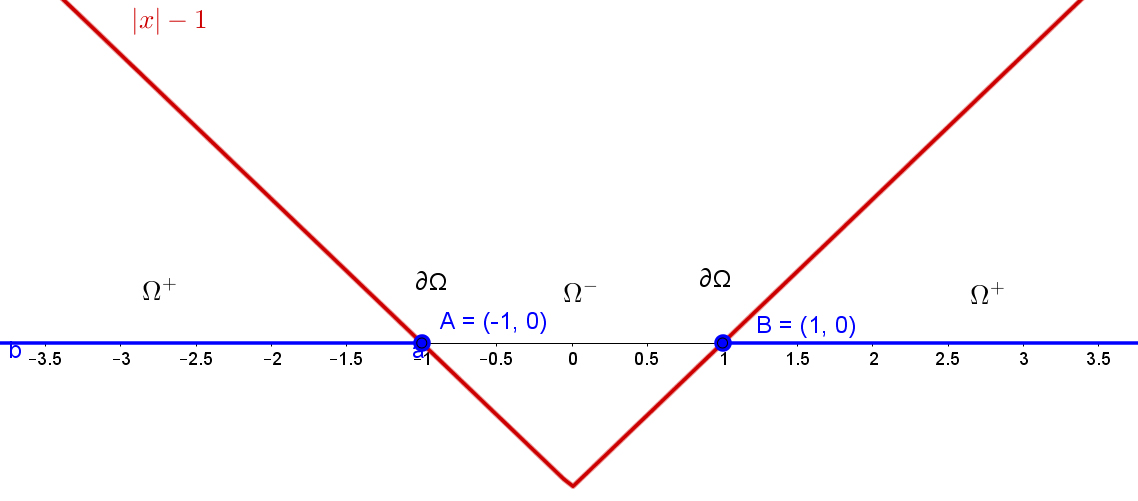
\includegraphics[width=0.6\textwidth]{revisao_bibliografica/signed_dist}
	\end{center}
	\legend{Modificado de \citeonline{osher}}
\end{figure}

Contextualizando, considere o furo de sondagem vertical interceptando uma camada de carvão, à direita na \autoref{carvao}, e o valor da função distância assinalada para essa litologia à esquerda. O valor da função decresce à medida que um ponto ao longo do furo se aproxima da camada, e seu valor é a menor distância desse ponto até um ponto pertencente à interface. Vale zero na interface, e passa a ser negativo para pontos no interior da camada, atingindo o menor valor no centro, parte mais interna da camada de carvão.

\begin{figure}[!htb]
	\caption{\label{carvao}Furo de sonda interceptando uma camada de carvão, à esquerda, e o valor da função distancia assinalada à direita.}
	\begin{center}
		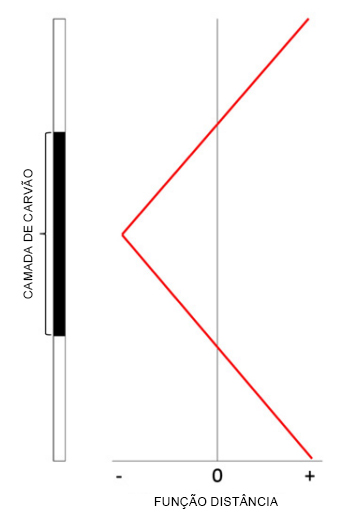
\includegraphics[width=0.2\textwidth]{revisao_bibliografica/carvao}
	\end{center}
	\legend{Modificado de \citeonline{deutschcoal}}
\end{figure}

Os exemplos apresentados são casos simplórios baseados em funções paramétricas e não são aplicáveis a características geológicas, embora a ideia central seja a mesma, algumas adaptações devem ser feitas para o emprego da técnica sob uma perspectiva geológica. A \autoref{metodologia} descreve como as funções implícitas devem ser construídas e aplicadas.

\section{Método implementado no \textit{software} \textit{Leapfrog}\textsuperscript{\textregistered}}\label{sec_leapfrog}

O assunto foi introduzido no campo da geologia por \citeonline{cowan2002rapid,cowan2003practical}, baseado no trabalho de \citeonline{savchenko} para modelar objetos através da interpolação de uma função implícita. 

O \textit{Leapfrog}\textsuperscript{\textregistered} permite a construção de modelos, geológicos e/ou de iso teores (\textit{grade shells}), tridimensionais a partir dos dados brutos de sondagem em questão de minutos ou horas, contra dias ou até semanas gastos com o método tradicional. Desse modo, diferentes cenários geológicos podem ser testados. Os modelos são gerados de forma semi automática. Ademais, informação geológica qualitativa pode ser incorporada ao modelo de forma prática e rápida \cite{cowan2002rapid}.
 
 \subsection{Metodologia}
 
Corpos geológicos são definidos implicitamente a partir dos dados de litologia provenientes da sondagem. O valor de uma função implícita (função distância assinalada ou função volume) é calculado para os pontos amostrais e interpolado para todo o espaço. Então, o volume que representa o corpo geológico é definido por uma iso superfície (geralmente a iso superfície zero) da função implícita interpolada \cite{cowan2003practical}. A metodologia para construção da função distância assinalada é elucidada na \autoref{metodologia}. Os corpos geológicos são modelados individualmente, em ordem geocronológica, do mais recente para o mais antigo, evitando a sobreposição de domínios. O \textit{Leapfrog}\textsuperscript{\textregistered} trabalha convertendo uma função implícita em uma superfície triangulada (\textit{mesh}) que representa a unidade geológica.

\subsubsection{Interpolação}

O exemplo a seguir, que ilustra a metodologia de interpolação implementada no \textit{software}, foi apresentado por \citeonline{leapfrogpredictions}.

\begin{figure}[!htb]
	\caption{\label{dk_amostras}Três amostras $s_1$, $s_2$ e $s_3$ e o um ponto $q$ a ser estimado.}
	\begin{center}
		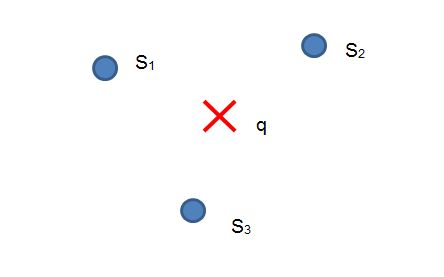
\includegraphics[width=0.4\textwidth]{revisao_bibliografica/dual_krig_amostras}
	\end{center}
	\legend{Fonte: \citeonline{leapfrogpredictions}}
\end{figure}

A \autoref{dk_amostras} ilustra o problema fundamental de estimar o valor $q$ a partir de três amostras $s_1$, $s_2$ e $s_3$.

A krigagem, em sua forma mais simples, estima o valor em um ponto como uma combinação linear das amostras conhecidas, os pesos são determinados matematicamente pela distribuição das amostras em relação ao ponto a ser estimado. Considerando o exemplo anterior:

\begin{equation}
q=w_1s_1+w_2s_2+w_3s_3
\end{equation}

Onde $w_1$, $w_2$ e $w_3$ são os pesos atribuídos às amostras.

Fica evidente que a krigagem pode ser usada como forma de interpolação, já que é possível estimar um valor em qualquer posição arbitrária onde não há dados. Todavia, para cada nova estimativa, é necessário recalcular os pesos, um processo que toma esforço computacional e tempo.

É possível rearranjar a equação de krigagem da seguinte forma:

\begin{equation}
q(x)=a_1\psi(x-x_1)+a_2\psi(x-x_2)+a_3\psi(x-x_3)
\end{equation}

Esse método é conhecido como \textit{dual kriging} \cite{galli1984dual}. $a_1\psi(x-x_1)$ descreve como a amostra localizada na posição $x_1$ influencia a estimativa na sua vizinhança, $\psi(x)$ é equivalente ao variograma (ou interpolante no casos das RBF). Nessa abordagem, as influências ponderadas de cada amostra são somadas para produzir uma equação que possa ser usada para estimar um valor em qualquer local $x$. Uma estimativa feita dessa maneira produz o mesmo resultado do que o método tradicional de krigagem. 

A \autoref{dk_pesos} ilustra um exemplo unidimensional do método

\begin{figure}[!htb]
	\caption{\label{dk_pesos}Demonstração simplificada do funcionamento das funções de bases radiais em uma dimensão.}
	\begin{center}
		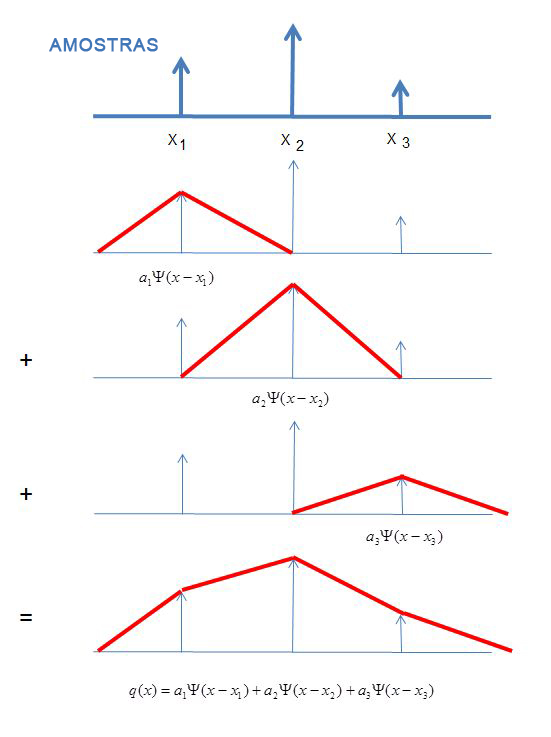
\includegraphics[width=0.4\textwidth]{revisao_bibliografica/dual_krig_pesos}
	\end{center}
	\legend{Modificada de \citeonline{leapfrogpredictions}}
\end{figure}

Utilizando a metodologia tradicional de krigagem, para cada nova estimativa em um local diferente é preciso recalcular os pesos, já com a \textit{dual kriging}, onde a influência das amostras é somada, os pesos só precisam ser calculados uma única vez. Acelerando o processo.

O \textit{Leapfrog}\textsuperscript{\textregistered} usa funções de bases radias (RBF) para interpolar a função distância assinalada retendo todas as amostras disponíveis (estimador global) em todas as estimativas. Mais especificamente \textit{FastRBF}\textsuperscript{TM}, cuja diferença principal em relação à RBF tradicional, é a capacidade de trabalhar com bancos de dados volumosos (mais de 1.000.000 de amostras) em um hardware convencional de forma relativamente rápida \cite{leapfrogfastrbf}. 

RBF são uma forma de implementar a \textit{dual kriging} \cite{leapfrogpredictions}. Enquanto a krigagem usa uma função covariância obtida através dos dados para determinar os pesos dados às amostras, as RBF usam funções básicas (\textit{interpolant functions}) pré-definidas para determiná-la.

Duas funções são usadas para derivar os pesos dados à cada amostra no \textit{Leapfrog}\textsuperscript{\textregistered}, o interpolante linear (\autoref{interpolantes} à esquerda) e o interpolante esferoidal (\autoref{interpolantes} à direita). Equivalentes aos modelos de variograma potência e esférico, respectivamente \citeonline{leapfrogbasics}.

O interpolante linear é multi escala, o que o torna bastante flexível e de uso geral. Particularmente recomendado para casos em que há um grande número de dados de litologia concentrados em bolsões localizados. Não é recomendado para teores, já que extrapola violentamente para além do limite dos dados. O interpolante esferoidal contorna o problema de extrapolação, muitas vezes não realista, do modelo linear \cite{leapfroginterpolant}.Os parâmetros do modelo como patamar, alcance e efeito pepita podem ser ajustados.

\begin{figure}[!htb]
	\caption{\label{interpolantes}Interpolantes do \textit{Leapfrog}\textsuperscript{\textregistered}.}
	\begin{center}
		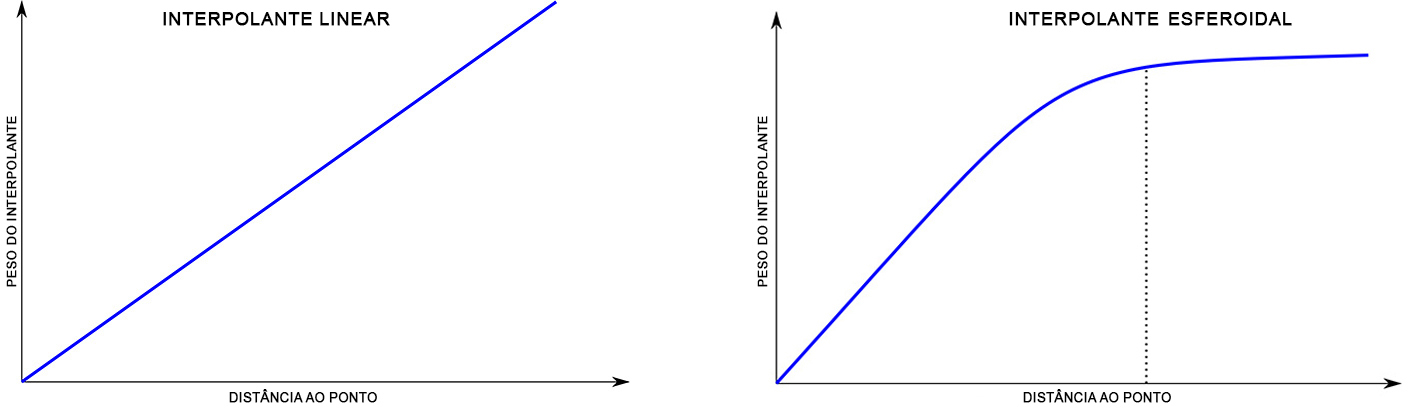
\includegraphics[width=0.8\textwidth]{revisao_bibliografica/interpolantes}
	\end{center}
	\legend{Modificada de \citeonline{leapfrogbasics}}
\end{figure}

\subsubsection{Anisotropia}

O \textit{Leapfrog}\textsuperscript{\textregistered} conta com ferramentas que dão ao usuário controle sobre a continuidade dos corpos geológicos em determinadas direções com possibilidade de incorporar à interpolação uma tendência global e/ou uma tendência estrutural.

A tendência global controla o comportamento do modelo interpolante, e deve ser utilizado em situações onde a geologia sugere continuidade do corpo numa direção planar sobre uma grande área, se a geologia sugerir que a direção dos corpos varia no espaço, a tendência estrutural é mais indicada \cite{leapfroganisglobal}.

A tendência global é inserida ao modelo a partir de um elipsoide de anisotropia, de forma análoga aos variogramas anisotrópicos da geoestatística.

A tendência estrutural é uma generalização da tendência global que permite alterar a direção de continuidade ao longo de uma superfície definida pelo usuário, ao invés de ser baseada em um plano, como a tendência global, definida a partir de um elipsoide de anisotropia. A tendência estrutural é baseada em uma superfície que pode apresentar qualquer forma e orientação, e é condicionada, geralmente, por restrições geológicas, como falhas, dobras, foliações... Para cada ponto da superfície (\textit{mesh}) definida, a tendência local é determinada, produzindo uma anisotropia que varia por todo o espaço definido \cite{leapfrogstructural}.

A tendência estrutural não determina a forma final da unidade geológica, ela é determinada pelo interpolante e pelas amostras retidas na interpolação. A \autoref{isotropico} mostra uma superfície interpolada usando um interpolante isotrópico, a \autoref{global} um interpolante com tendência global e a \autoref{estrutural} um interpolante com tendência estrutural. Todos os sólidos derivam da mesma base de dados.

\begin{figure}[!htb]
	\caption{\label{isotropico}Interpolante isotrópico.}
	\begin{center}
		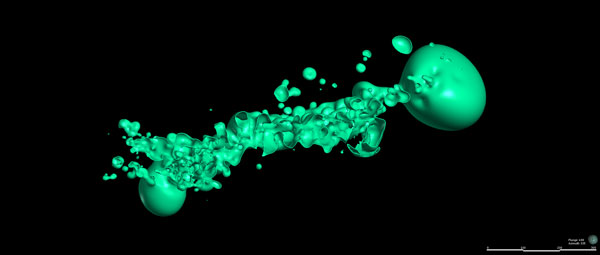
\includegraphics[width=0.5\textwidth]{revisao_bibliografica/isotropic_interpolant}
	\end{center}
	\legend{Fonte: \citeonline{leapfrogstructural}}
\end{figure}

\begin{figure}[!htb]
	\caption{\label{global}Tendência global aplicada ao interpolante.}
	\begin{center}
		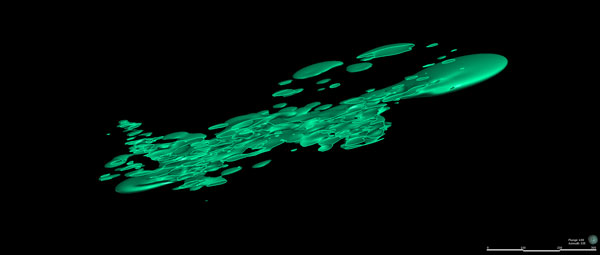
\includegraphics[width=0.5\textwidth]{revisao_bibliografica/global_trend_interpolant}
	\end{center}
	\legend{Fonte: \citeonline{leapfrogstructural}}
\end{figure}

\begin{figure}[!htb]
	\caption{\label{estrutural}Tendência estrutural aplicada ao interpolante.}
	\begin{center}
		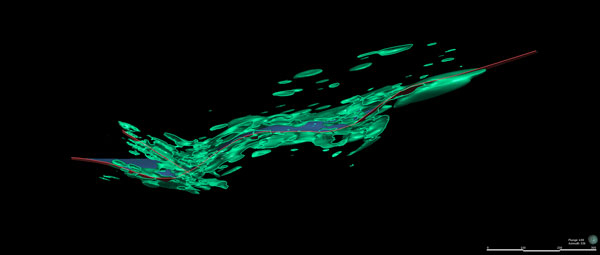
\includegraphics[width=0.5\textwidth]{revisao_bibliografica/structural_trend_interpolant}
	\end{center}
	\legend{Fonte: \citeonline{leapfrogstructural}}
\end{figure}

O \textit{Leapfrog}\textsuperscript{\textregistered} disponibiliza três tipos de tendência estrutural (\textit{non-decaying trends}, \textit{blended trends} e \textit{strongest along meshes}), que compartilham os mesmos parâmetros força (\textit{strength}) e alcance (\textit{range}). A força é semelhante à razão do elipsoide e dita quanta elongação existirá em uma determinada direção. Enquanto o alcance dita até que distância da superfície definida (\textit{mesh}) a tendência ainda tem efeito \cite{leapfrogstructural}.  

\subsubsection{Visão geral}

A metodologia do \textit{Leapfrog}\textsuperscript{\textregistered} compreende cinco passos \cite{cowan2002rapid}:
\begin{enumerate}
\item Validação dos dados e compositagem: Esse passo pode ser executado na maior parte dos software de mineração disponíveis;
\item Interpolação e \textit{meshing}: Extrair iso superfícies de uma função distância assinalada interpolada;
\item Incorporar geomorfologia: estruturas geológicas interpretadas pelo geomodelador são inseridas no modelo como tendência estrutural;
\item Interpolação da informação morfológica: Uma função de interpolação é ajustada à informação digitalizada no passo anterior;
\item Interpolação condicionada à informação geomorfológica: A interpolação do segundo passo é repetida, dessa vez, condicionada pela função de interpolação da informação morfológica gerada no quarto passo. Essa etapa gera modelos que honram os dados amostrais, e são consistentes com a informação qualitativa interpretada pelo geomodelador.
\end{enumerate}

A metodologia implementada no \textit{leapfrog}\textsuperscript{\textregistered} supera muitas das limitações dos métodos explícitos. Os domínios são construídos de forma rápida, o método é objetivo, replicável e nova informação geológica pode ser incorporada facilmente aos modelos. O \textit{software} conta com funções interessantes como a possibilidade de inserir no modelo informação geológica qualitativa e ferramentas específicas para modelar estruturas geológicas complexas como diques. No entanto, o fato da RBF ser um interpolador global pode inviabilizar o uso do método em bancos de dados muito grandes, o método não trabalha com múltiplos domínios de forma direta e sua licença é bastante cara \cite{mclennan2006implicit}.

\section{Método dos campos potenciais}\label{sec_campos}

O método dos campos potenciais, implementado no \textit{software Isatis} \textsuperscript{\textregistered}, foi criado para construir modelos geológicos tridimensionais a partir de dados de geologia e de exploração \cite{chiles2004modelling}. O princípio do método é derivar a geometria dos domínios a partir da interpolação tridimensional de um campo escalar, conhecido como campo potencial. O campo potencial é construído através da cokrigagem da informação dos contatos geológicos provenientes de furos de sondagem e dados estruturais \cite{renard2013modeling}.

A localização dos contatos estabelece a posição de referência de iso valores do campo potencial enquanto os dados de orientação são o gradiente da função escalar (campo potencial). A geometria dos corpos geológicos é obtida a partir da discretização de iso valores de referência \cite{calcagno2008geological}, semelhante a como uma unidade geológica é definida a partir de uma iso superfície de uma função implícita nos métodos apresentados na \autoref{sec_leapfrog} e \autoref{metodologia}. 

A covariância da cokrigagem e o gradiente do campo potencial estimado podem ser transformados em medidas de incerteza da localização da fronteira dos domínios ou usadas para mapear a probabilidade de um local não amostrado pertencer a um determinado domínio geológico \cite{renard2013modeling}.

\subsection{Metodologia}

O método consiste em modelar uma interface geológica ou uma série de interfaces sub paralelas $l_k$, $k=1,2,...$. Seu princípio é sumarizar a geologia a partir de um campo potencial, isto é, uma função escalar $T(p)$ de qualquer ponto $p=(x,y,z)$ no espaço tridimensional, a interface $l_k$ corresponde a uma superfície iso potencial, ou seja, o conjunto de pontos $p$ que satisfazem $T(p)=t_k$ para algum valor desconhecido $t_k$ do campo potencial. De forma análoga, a formação geológica entre duas interfaces sucessivas $l_k$ e $l_{k'}$ é definida por todos os pontos $p$ os quais o campo potencial pertence ao intervalo definido por $t_k$ e $t_{k'}$ \cite{chiles2004modelling}. 

A \autoref{pot_field_1} ilustra o princípio em duas dimensões. À esquerda, uma formação geológica foi mapeada pela posição de suas interfaces com outras duas formações (pontos vermelhos e azuis) e medidas do mergulho (setas). À direita, a formação geológica foi modelada pelo método dos campos potenciais, curvas vermelhas e azuis representam iso valores de referência dos contatos modelados. Curvas brancas são iso valores selecionados do campo potencial, e representam tendências geológicas ou trajetórias de foliações. As interfaces honram tanto os pontos pertencentes aos contatos quanto os vetores de orientação \cite{calcagno2008geological}.

\begin{figure}[!htb]
	\caption{\label{pot_field_1}Princípio do método dos campos potenciais em duas dimensões.}
	\begin{center}
		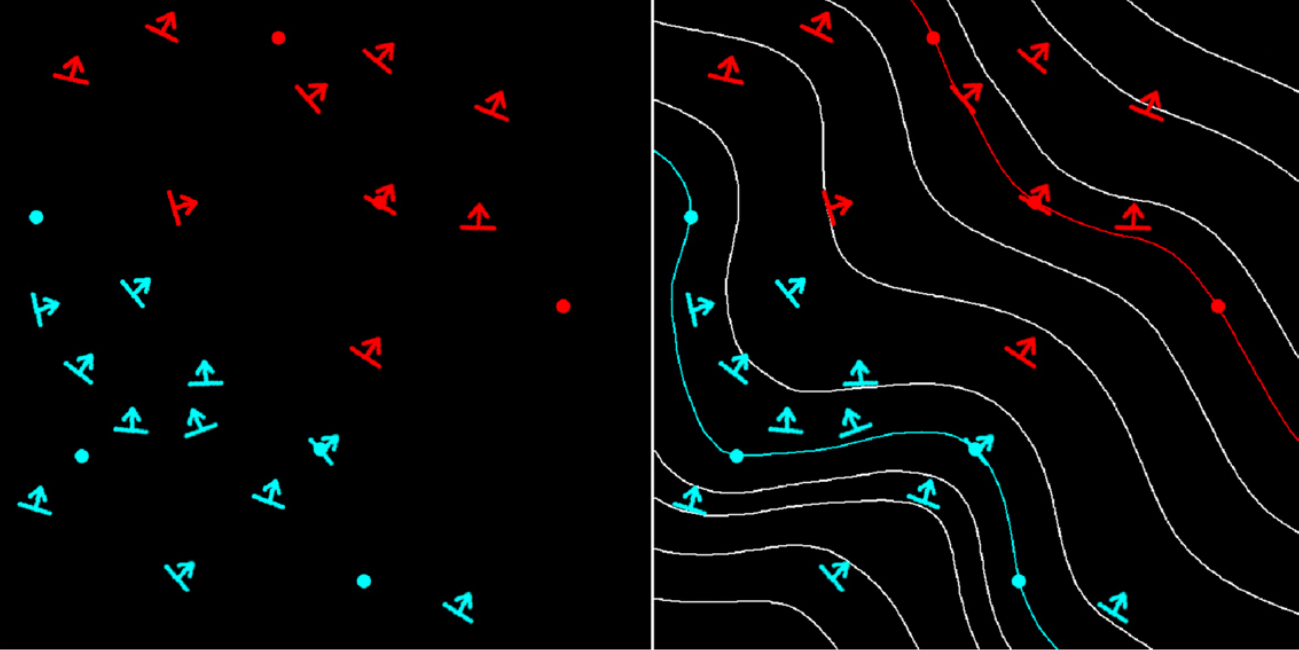
\includegraphics[width=0.8\textwidth]{revisao_bibliografica/pot_field_1}
	\end{center}
	\legend{Fonte: \citeonline{calcagno2008geological}}
\end{figure}

\subsection{Tipos de dados}

$T(p)$ é modelada com dois tipos diferentes de dados \cite{chiles2004modelling}:

\begin{enumerate}
\item Coordenadas tridimensionais de pontos que pertencem às interfaces $l_1, l_2, ...$ (contatos geológicos);
\item Vetores unitários tridimensionais que pertencem ao campo de orientação das interfaces.  
\end{enumerate}

Na modelagem tridimensional de interfaces sedimentares, a informação estrutural consiste em vetores unitários ortogonais ao principal plano de anisotropia (acamamento, xistosidade, foliação) e apontando no sentido das formações mais jovens. Na modelagem de um domínio mineralizado, os vetores unitários apontam do interior para o exterior dos domínios \cite{renard2013modeling}.

\subsubsection{Codificação dos dados}

Para interpolar o campo potencial, os dados devem ser codificados da seguinte forma \cite{chiles2004modelling, calcagno2008geological, renard2013modeling}:


\begin{enumerate}
\item Pontos da interface: O valor potencial $c$ associado com a interface não é conhecido, mas a diferença potencial entre dois pontos de uma interface é igual a zero (já que as superfícies são equipotenciais). Os $m+1$ pontos $p_0, p_1, ..., p_m$ da interface são transladados em $m$ incrementos $T(p_{\alpha})-T(p'_\alpha)=0$, $\alpha=1,...,m$. $p'_\alpha$ pode ser tanto o ponto $p_0$ ou o ponto $p_{\alpha-1}$ (a escolha não tem impacto no resultado);
\item Dados de orientação: Os vetores unitários normais a cada plano estrutural, são considerados como gradiente do campo potencial, equivalentes ao valor da derivada parcial $\frac{\partial T(p)}{\partial u}$ no ponto medido $p_\beta$ em qualquer direção $u$. O dado estrutural em $p_\beta$ pode ser escrito como três derivadas parciais da forma $\frac{\partial T(p_\beta)}{\partial u_\beta}$, $u_\beta$, representando os eixos de coordenadas $x, y, z$ (um outro conjunto de derivadas parciais em três direções ortogonais também pode ser considerado. Por exemplo, o vetor unitário pode ser expressado por uma derivada parcial igual a um na direção do vetor, e duas derivadas parciais iguais a zero nas direções que definem o plano estrutural).    
\end{enumerate}

\subsubsection{Interpolação do campo potencial}

A função potencial $T(.)$ é definida até uma constante arbitrária que é o potencial em um ponto de referência arbitrário $p_0$. Em cada ponto $p$ o incremento do campo potencial $T(p)-T(p_0)$ é krigado. O estimador de cokrigagem é escrito como:

\begin{equation}
	\label{eq_pot_field}
    T^*(p)-T^*(p_0)=\sum\limits_{\alpha=1}^M \mu_\alpha(T(p_\alpha)-T(p'_\alpha))+\sum\limits_{\beta=1}^N \nu_\beta \frac{\partial T(p_\beta)}{\partial u_\beta}
\end{equation}

Onde os pesos $\mu_\alpha$ e $\nu_\beta$, determinados pelo sistema de cokrigaem, são função de $p$ (e $p_0$). Embora a contribuição dos incrementos potenciais seja zero, os pesos $\nu_\beta$ são diferentes dos pesos baseados apenas nos dados de gradiente.

A cokrigagem é estabelecida sob o modelo de função aleatória (\autoref{func_al}). $T(.)$ é assumido como uma função aleatória com deriva (\textit{drift}) polinomial $m(p)$:

\begin{equation}
	\label{eq_poli_drift}
    m(p)=\sum\limits_{l=0}^L b_lf^l(p)
\end{equation}

E uma variância estacionária $K(h)$ \cite{calcagno2008geological,renard2013modeling}. Uma vez que as funções básicas $f^l(p)$ da deriva e a covariância $K(h)$ de $T(.)$ sejam conhecidas, a cokrigagem, na presença de dados do gradiente, pode ser calculada. Já que a derivada de $\frac{\partial T(p)}{\partial u}$ vale $\frac{\partial m(p)}{\partial u}$, isto é, uma combinação linear das derivadas parciais $\frac{\partial f^l(p)}{\partial u}$ com os mesmos coeficientes desconhecidos $b_l$ de $m(p)$. As covariâncias das derivadas parciais são derivadas parciais de segunda ordem de $K(.)$, e as covariâncias cruzadas entre campo potencial e as derivadas parciais são derivadas parciais de $K(.)$ \cite{chiles2004modelling}.

\subsubsection{Implementação do algoritmo de cokrigagem}

O incremento dos dados potenciais não contribuem com as estimativas finais. O estimador pode ser visto como integração dos dados de gradiente \cite{chiles2004modelling}. Para garantir a continuidade espacial do estimador, é usada apenas uma vizinhança incluindo todos os dados. Quando não há interesse na variância, a cokrigagem é implementada em sua forma \textit{dual} (\textit{dual kriging}), assim, o sistema de krigagem é resolvido uma única vez. 

$T^*(p)-T^*(p_0)$ pode ser obtido em qualquer ponto. Seu sinal indica onde $p$ está localizado, negativo para formações mais antigas, positivo para formações mais recentes e zero para a interface. Essa propriedade permite a visualização em três dimensões do modelo geológico a partir de um algoritmo de cubos marchantes (\textit{marching cubes}) \cite{lorensen1987marching}, que rastreia a iso superfície do campo potencial \cite{calcagno2008geological}.

\subsubsection{Variância do campo potencial}

Na geoestatística, a covariância ou variograma de uma variável são modeladas a partir dos dados. Porém, não há medidas do potencial $T(x)$, e os incrementos potenciais usados na interpolação não podem ser usados na inferência de $K$, já que todos valem zero.

Na sua primeira implementação, o algoritmo era baseado em um modelo de covariância arbitrariamente escolhido pelo usuário \cite{chiles2004modelling}.

Quando existem muitos dados estruturais disponíveis, o variograma das derivadas parciais pode ser calculado. Os variogramas das derivadas parciais são derivadas de segunda ordem do variograma do campo potencial. \citeonline{renard2013modeling} recomenda que uma soma de modelos anisotrópicos cúbicos de covariância sejam adotados para modelar a covariância.

\subsubsection{Incerteza nos modelos}

Uma formação geológica definida pelo conjunto de pontos $p$ tais que $T(p)-T(p_0)$ está compreendido entre os dois valores $t$ e $t'$. Sob a suposição de que o campo potencial é uma função aleatória gaussiana, a probabilidade de um dado ponto $p$ pertencer à essa formação é:

\begin{equation}
\begin{gathered}
 P\{t \leq T(p)-T(p_0) < t'\}= \\ 
 G\left(\frac{t'-(T^*(p)-T^*(p_0))}{\sigma_{CK}(p)} \right) - G\left(\frac{t-(T^*(p)-T^*(p_0))}{\sigma_{CK}(p)} \right)
\end{gathered}
\end{equation}

Onde G é a função de distribuição acumulada normal.

De forma análoga, para a interface que passa por $p_0$ 

\begin{equation}
	R(p) = T(p)-T(p_0)=\frac{T^*(p)-T^*(p_0)}{\sigma_{CK}}
\end{equation}

Mede a probabilidade de $p$ pertencer à interface.

\subsubsection{Visão geral}

A metodologia compreende cinco passos \cite{mclennan2006implicit}:

\begin{enumerate}
\item Coletar dados de interseção e dados de orientação em superfície;
\item Determinar a forma da deriva (\textit{drift}) localmente variável;
\item Inferir a função covariância do campo potencial;
\item Interpolar o campo potencial com cokrigagem;
\item Visualizar a incerteza na localização das fronteiras estimadas.
\end{enumerate}

O método ainda permite a incorporação de falhas e informação geofísica. É um método flexível, que incorpora uma gama de dados diferentes na modelagem dos domínios geológicos. É rápido, em comparação com os métodos explícitos, é objetivo e replicável. Capaz de produzir modelos bastante complexos como o da \autoref{pot_field_ex}. Porém, o procedimento não é simples. É difícil inferir a covariância dos campos potenciais já que não existem dados amostrais do campo. As medições de orientações nem sempre existem ou são de fácil obtenção. O método etá implementado apenas em software pago.

\begin{figure}[!htb]
	\caption{\label{pot_field_ex}Modelo geológico criado a partir do método dos campos potenciais, em planta (acima). Seção N6 (abaixo).}
	\begin{center}
		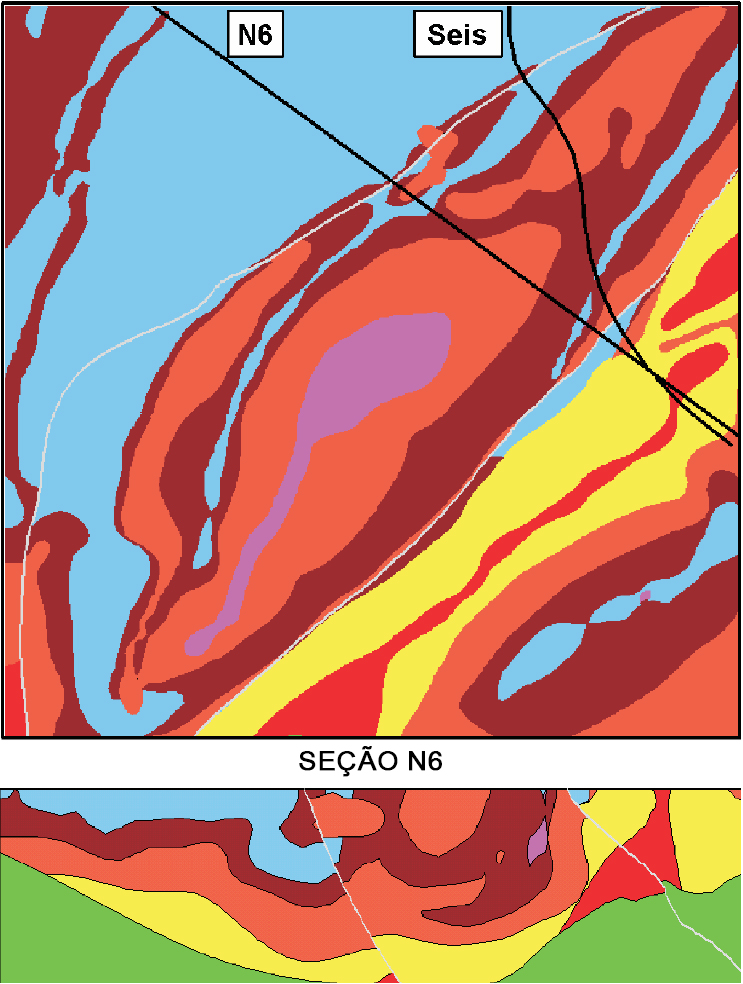
\includegraphics[width=0.5\textwidth]{revisao_bibliografica/pot_field_ex}
	\end{center}
	\legend{Fonte: \citeonline{chiles2004modelling}}
\end{figure}